\section{Liveness Bug in Azure Storage vNext}
\label{sec:cases:azurestore}

It took only tens of seconds before the testing harness reported the first occurrence of a liveness bug. Upon examining the debug trace, the vNext developers were able to confirm the bug.

However, the trace didn't include enough details, which prevented the developers from identifying a root cause. Fortunately, running the test harness took very little time, so the developers were able to quickly iterate and add more refined debug outputs in each iteration. After several iterations, the developers were able to pinpoint the exact culprit and immediately proposed a solution to fix the bug. Once the proposed solution was implemented, the developers again ran the testing harness, which reported no more bug for $100,000$ iterations in tens of minutes.

The liveness bug occurs in the second testing scenario, where the \texttt{TestingDriver} fails one of the \texttt{ExtentNode} and launches a new one. The \texttt{RepairMonitor} transitions to the hot repairing state and is stuck in the state for infinitely long.

Here is one particular execution sequence resulting in the bug. $i)$ EN$_0$ fails and is detected by the EN expiration loop; $ii)$ EN$_0$ is removed from the EN map; $iii)$ the extent center is updated and the replica count drops from 3, the target, to 2; $iv)$ \texttt{ExtMgr} receives a sync report from EN$_0$; $v)$ the extent center is updated and the replica count increases from 2 to 3 again. This is problematic because, on one hand, the replica count is equal to the target, so the extent repair loop never schedules any repair task. On the other hand, there are only two true replicas in the system, one fewer than the target. This execution sequence leads to one replica missing. Conceivably, repeating this another two times would result in all replicas missing, while \texttt{ExtMgr} still thinks all replicas are healthy. If deployed in production, such bug would have caused a very serious incident of customer data loss.

The culprit is in $iv)$, where \texttt{ExtMgr} receives a sync report from EN$_0$ after deleting the EN. This may occur in \psharp because of arbitrary message interleaving. It may also occur, albeit much less frequently, in the stress testing due to messages being delayed in the network. This explains why the bug only occurs from time to time in the stress testing and also takes long execution to trigger. In contrast, \psharp allows the bug to manifest quickly, the developers to iterate rapidly, the culprit identified promptly, and the fix solution verified effectively, all of which should vastly increase the productivity of distributed storage system development. 

\section{Additional Example I: Live Azure Table Migration}
\label{sec:cases:migration}

The Live Azure Table Migration is a library capable of transparently migrating a data set between tables in the Windows Azure storage service while an application is accessing the data set.  MigratingTable provides a \emph{virtual table} with an API similar to that of an ordinary Azure table, backed by a pair of \emph{old} and \emph{new} tables.  A background \emph{migrator} job moves all data from the old table to the new table.  Meanwhile, each read or write issued to the virtual table is translated to a sequence of reads and writes on the backend tables according to a protocol we designed, which guarantees linearizability of operations on the virtual table across multiple application processes assuming that the backend tables respect their own linearizability guarantees.

\begin{figure}[t]
\centering
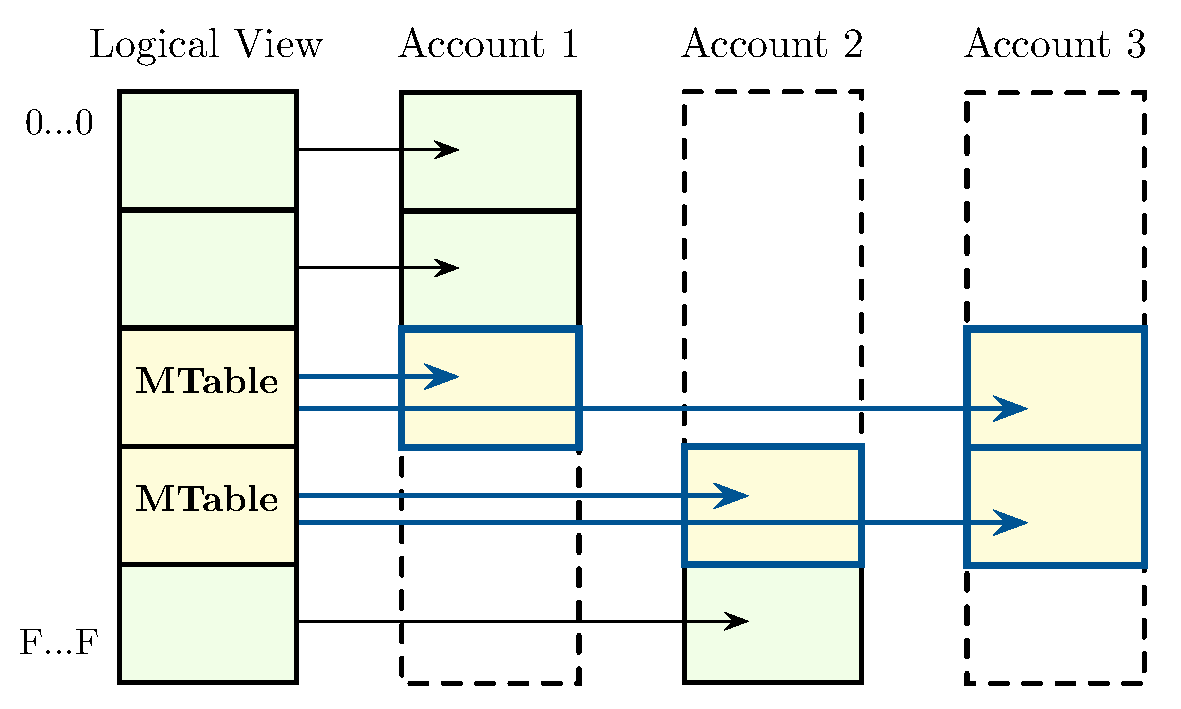
\includegraphics[width=\linewidth]{img/livemigration}
\caption{Resharding a data set when a third Azure storage account is added. Two key ranges are each migrated to the new account using a MigratingTable instance (abbreviated MTable).}
\label{fig:livemigration}
\end{figure}

% N.B. Artifact Services is mentioned at http://research.microsoft.com/en-us/people/schulte/.  Hopefully it's OK to reveal that it was the system in this case study. ~ Matt 2015-08-17
The initial motivation for MigratingTable was to solve a scaling problem for Artifact Services, an internal Microsoft system with a data set that is sharded across tables in different Azure storage accounts because it exceeds the limit on traffic supported by a single Azure storage account.  As the traffic continues to grow over time, the system needs to reshard the data set across a greater number of Azure storage accounts without interrupting service.  During such a resharding, our sharding manager will identify each key range that should migrate to a different table, and we will use a separate MigratingTable instance for each such key range to actually perform the migration (Figure~\ref{fig:livemigration}).  MigratingTable may also be useful to migrate data to a table with different values of configuration parameters that Azure does not support changing on an existing table, such as geographic location.

\def\term#1{\emph{#1}}
We also used \psharp to test the MigratingTable library, which is capable of transparently migrating a data set between tables in the Windows Azure storage service while an application is accessing the data set.

\begin{figure}[t]
\centering
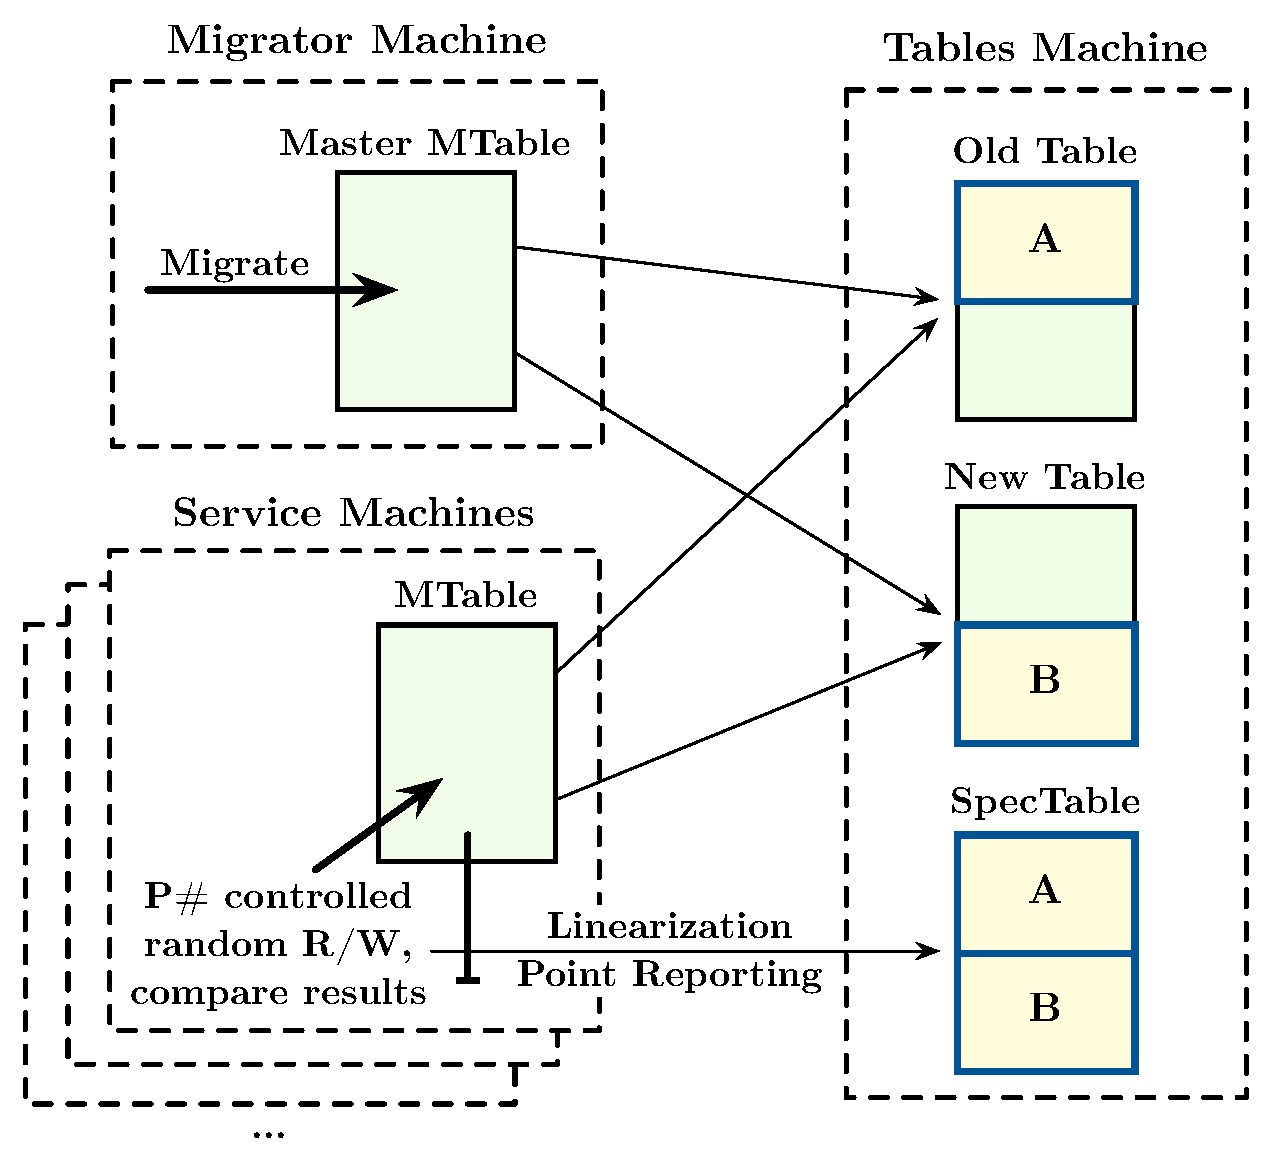
\includegraphics[width=\linewidth]{img/mocked_migration}
\caption{MigratingTable \psharp correctness test environment.}
\label{fig:mockedmigration}
\end{figure}

Since we were designing a new concurrent protocol that we expected to become increasingly complex over time as we add optimizations, we planned from the beginning to maintain a \psharp test harness along with the protocol to maintain confidence in its correctness.

MigratingTable implements an interface called IChainTable2, which provides the core read and write functionality of the original Azure table API with one exception: it provides \term{streaming reads} with a weaker consistency property than multi-page reads in the original API, since the original property would have been difficult to achieve for no benefit to applications we could foresee.  MigratingTable requires that its backend tables also implement IChainTable2, and we wrote a simple adapter to expose physical Azure tables as IChainTable2.  Our goal was then to verify that when multiple application processes issue ``input'' read and write calls to their own MigratingTable instances with the same backend tables, the behavior complies with the specification of IChainTable2 for the combined input history.

\subsubsection{Input generation}
\label{sec:mtable:input}

% N.B. SpecTable = InMemoryTableWithHistory in the current codebase. ~ Matt 2015-08-17
Of course, there are many possible input histories for MigratingTable.  We could have tested specific input histories, but we were not confident that this approach would be effective in catching bugs, especially because concurrency increases the potential for interactions between different parts of the code that would be difficult for us to foresee.  If we had no formalization of the specification and had to rely on expected outputs worked out by hand, this might be the best we could do.  However, since the IChainTable2 specification is relatively simple and is almost deterministic under sequential calls, it was straightforward to write an in-memory reference implementation called SpecTable to which we can compare the output of MigratingTable on an arbitrary input history.  This gave us the attractive option to sample from a distribution we defined over all possible input histories within certain bounds.  It was convenient to let \psharp control the choice of input history as well as the schedule so we could reproduce both using a single random seed.  Then, under the ``small scope hypothesis'' that any bug in MigratingTable leads to incorrect output for at least one input history in our distribution, we have a positive probability of detecting this incorrect output on each iteration of the \psharp test.

All of our input histories include two application processes.  Each process performs either a single streaming read or a sequence of two atomic calls, each a read or a batch write.  Each batch write call includes one or two operations, where the operation type is chosen from the set supported by IChainTable2 (Insert, Replace, Merge, Delete, InsertOrReplace, InsertOrMerge, DeleteIfExists) and the row key is chosen from $\{0, \ldots, 5\}$.  If the operation requires an If-Match value, it is equally likely to be \texttt{*}, the current ETag of the row (if it exists), or some non-matching value.  Finally, the new entity includes a user-defined property \texttt{isHappy} whose value is equally likely to be true or false.  For both atomic and streaming reads, the filter expression is equally likely to be empty (i.e., match everything), \texttt{isHappy eq true}, or \texttt{isHappy eq false}.

\subsubsection{Model structure}

As mentioned above, the IChainTable2 specification is almost deterministic under sequential calls; the only nondeterminism is in the results of streaming reads.  Given a streaming read, SpecTable can compute the set of all results that are compliant with the specification, so we can simply check if the result of MigratingTable is in this set.  To test MigratingTable, we must supply it with backing tables.  We use SpecTable for this purpose as well, with \psharp choosing the actual result of each streaming read from the valid set.  Our correctness property is then:
% Convert to some theorem-like environment? ~ Matt
\begin{quote}
For every execution trace of a collection of MigratingTables backed by the same pair of \term{old} and \term{new} SpecTables in parallel with the migrator job, there exists a linearization of the combined input history such that the output in the original trace matches the output of a ``reference'' SpecTable on the linearized input.
\end{quote}
%
We instrumented MigratingTable to report the intended \term{linearization point} of each input call, which in our setting is always one of the corresponding \term{backend calls} to the backend tables (often the last).  Specifically, after each backend call completes, MigratingTable reports whether that call was the linearization point, which may depend on the result of the call.  This makes it possible to verify the correctness property as the model executes.  The model consists of a \psharp \term{tables machine} containing all three SpecTables; a collection of \term{service machines} containing identically configured MigratingTables; and a \term{migrator machine} that performs the background migration (Figure~\ref{fig:mockedmigration}).  Each service machine issues a random sequence of input calls to its MigratingTable, which sends backend calls to the tables machine.  When MigratingTable reports the linearization point of an input call, the service machine sends that input call to the reference table.  When an input call completes, the service machine checks that the results from the MigratingTable and the reference table agree.  \psharp controls the interleaving of the backend calls.  To ensure that the reference table is never observed to be out of sync with the backend tables, after the tables machine processes a backend call, it enters a state that defers further backend calls until MigratingTable has reported whether the backend call was a linearization point and (if so) the call to the reference table has been made.  We use the \psharp random scheduling strategy; we were afraid that an exhaustive strategy would only be feasible within bounds so low that we would miss some bugs.

We wanted to implement the core MigratingTable algorithms in \csharp ``async/await'' code, like most of Artifact Services, to achieve both good readability and good performance.  We used a method similar to that described in Section~\ref{sec:psharp:async} to bring the generated TPL tasks under the control of the \psharp scheduler.  Then we implemented an ``async'' RPC mechanism based on the .NET RealProxy class that automates the generation of proxies for objects hosted by other \psharp machines (in our setting, the service machines use proxies for the SpecTables and various auxiliary objects hosted by the tables machine).  When a machine calls a method on a proxy, the proxy sends a \psharp message to the host machine, causing it to execute the method call on the original object and send back the result, which the proxy then returns.  Thus, the use of these proxies as IChainTable2 backends is transparent to the MigratingTable library, thanks to dynamic dispatch.

\subsection{An example bug in MigratingTable}
\MMComment{Move wherever appropriate}

One of the bugs in MigratingTable that we found using the \psharp test stands out because it reflects the type of oversight that tends to occur as designs evolve and it's unclear whether we would have been able to find it by any other method (\MMComment{revise remark when we have stress test results?}).  This bug, which we named QueryStreamedBackUpNewStream, is in the implementation of a streaming read from the virtual table, which should return a stream of all rows in the table sorted by key.  The essential implementation idea is to start streams $s_O$, $s_N$ from the old and new backend tables and merge the sorted streams by keeping track of the next row in each stream and returning the row with the lesser key.  In parallel, the migrator job is concurrently copying rows from the old table to the new table; we had satisfied ourselves that this concurrency would not cause any problems.  However, then we added support to the migrator job to delete the old table when it finishes copying, which triggers the virtual stream to close $s_O$.  Suppose the virtual stream is in a state in which the next row in $s_O$ has key $k_O$ and the next row in $s_N$ has key $k_N$, where $k_O < k_N$.  Further suppose that before the next read from the virtual stream, the migrator job copies a row with key $k$ ($k_O < k < k_N$) from the old table to the new table and then deletes the old table.  Since $s_O$ has not yet returned this row when it is closed and $s_N$ has already advanced to $k_N$, the row with key $k$ will be missed by the virtual stream.  A similar problem can occur if $s_N$ does not reflect rows inserted into the new table by the migrator job after $s_N$ is started, as allowed by the IChainTable2 specification.  Restarting $s_N$ when the old table is deleted fixes both variants of the bug.

% It might be nice to include excerpts of a trace like in migration-bug3-explanation.pptx.  Unfortunately, the trace in migration-bug3-explanation.pptx doesn't match my recollection of the original diagnosis, which I want to write about truthfully (the former looks like it involves a stale streaming read, while I'm fairly sure the latter involved only the $k_O < k < k_N$ case).  If it's important, I could try to get a new trace consistent with the original diagnosis. ~ Matt
This bug took us only about 10 minutes to diagnose from the trace; granted, this is after we had days of experience analyzing MigratingTable traces and had added our own trace output to the test harness, since \psharp's built-in trace output is too low-level and does not include event payloads and other diagnostic data that is not passed between machines.  We started from the failure symptom: the virtual stream returned end-of-stream when according to the reference SpecTable, it should have returned an additional row with key 4.  We filtered the trace for actions by the same service machine and saw that $s_O$ was closed before the virtual stream had returned the row with key 4, but $s_N$ had already advanced past key 4 before the migrator inserted the row in the new table.  At first we found this phenomenon hard to believe, but soon we were convinced it reflected a gap in our design.

\MMComment{Add a figure based on migration-bug3-explanation.pptx (probably a hybrid of slides 4 and 5, assuming we want only one figure).}

\section{Additional Example II: Azure Service Fabric (change to CScale?)}
\label{sec:cases:fabric}

\PDComment{I guess we should write stuff about CScale here based on our last discussion: overview of the system (collection of Fabric services connected via TPL dataflow?), of its environment (Fabric), how they interop?, why its very challenging to test? how they test currently? I am not sure if all these should go here or be split here and the experience report, we will see ... same for the above case studies}

\emph{Azure Service Faric} (or \emph{Fabric} for short) is a platform and API for creating reliable services that execute on a cluster of machines. The developer writes a service that receives requests (e.g.\ from some client program via HTTP requests) and mutates its state based on these requests. In order to make the service \emph{reliable}, Fabric launches several copies (\emph{replicas}) of the service, where each copy runs as a separate process on a different node in the cluster. One replica is selected to be the \emph{primary} which serves client requests; the rest are \emph{secondaries}. The primary replicates state changes to the secondaries by sending \emph{replication requests} so that all replicas eventually have the same state. If the primary fails (e.g.\ if the node on which the primary is running crashes), Fabric elects one of the secondaries to be the new primary and launches another secondary; the new secondary will receive a full or partial copy (depending on whether persistent storage is used) of the state of the new primary in order to ``catch up'' with the other secondaries. Fabric provides a name-resolution service so that clients can always find the current primary. 

Fabric services have a lot of asynchrony, which make them interesting targets for systematic testing with \psharp{}.
Our primary goal was to create a \psharp{} model of Fabric to allow
thorough testing of services, where Fabric's asynchrony is controlled 
by the \psharp{} runtime.
The system that we wished to test is \emph{CScale}~\cite{X},
a big data-stream processing system that chains multiple Fabric services
in a directed acyclic graph.
Prior work~\cite{deligiannis2015psharp}
created a model of Fabric with limited functionality;
it used a mixture of \csharp{} and \psharp{} internally,
only supported one in-flight replication request
(which restricts the asynchrony that can be tested),
and only supported one Fabric service.
Our new Fabric model was re-written to use only \psharp{}
internally,
support an arbitrary number of Fabric services and in-flight replication requests,
and in general be a more complete model of Fabric.
Note that \csharp{} code is still required to interface with the existing
\csharp{} service code.
We refer to our \csharp{} code
as the \emph{translation layer}
and
 the user-written \csharp{} service code as \emph{user code}. 

\begin{figure}[thb]
\centering
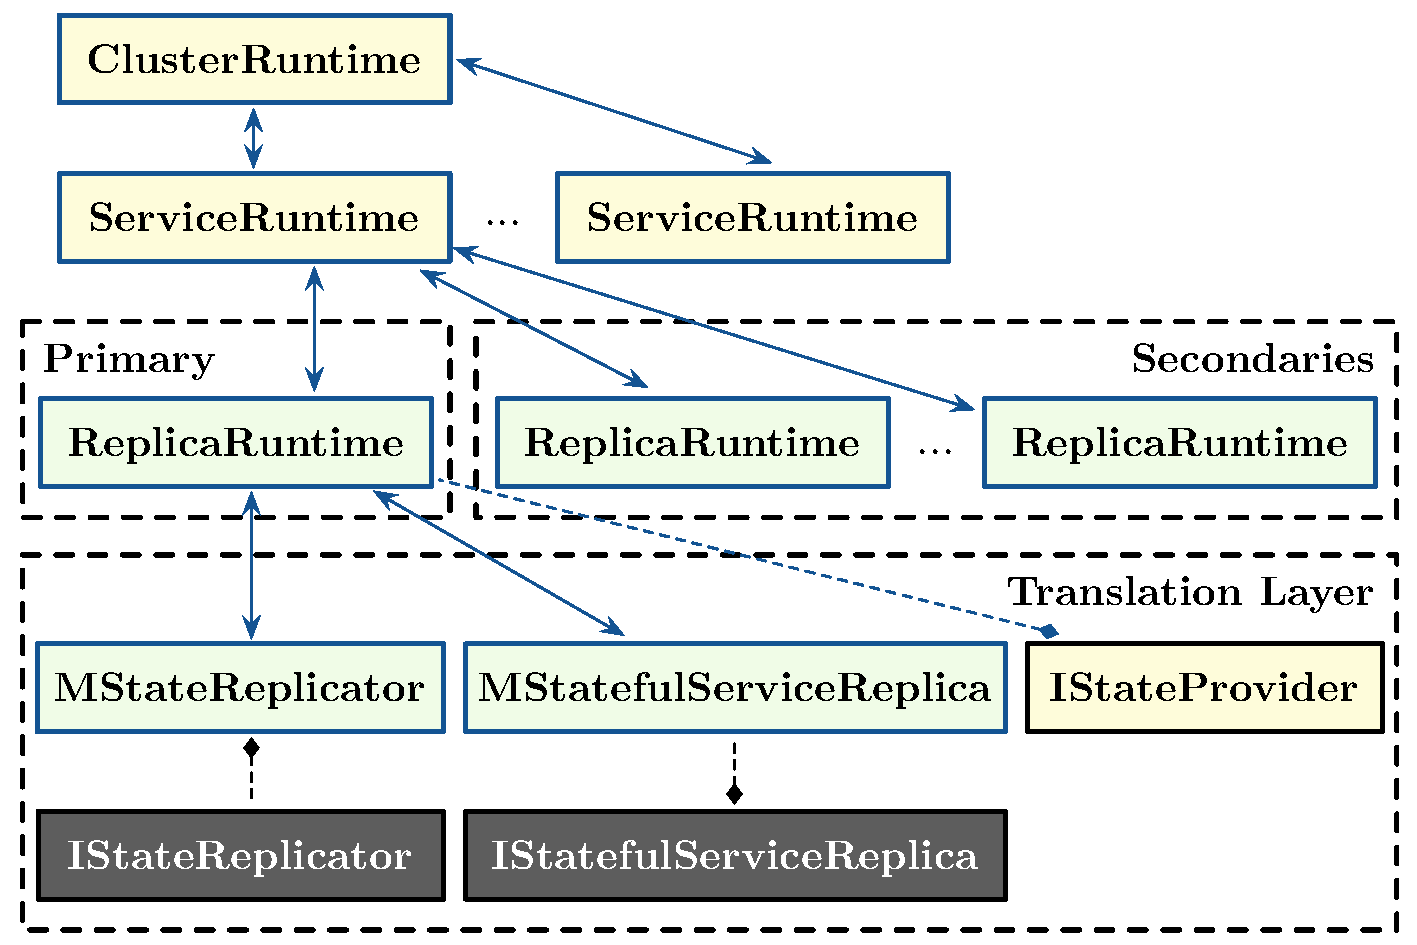
\includegraphics[width=\linewidth]{img/fabricmodel}
\caption{Overview of the key machines and interfaces in our Fabric model.}
\label{fig:fabric_model}
\end{figure}

An overview of our Fabric model is shown in Figure~\ref{fig:fabric_model}.
The \texttt{ClusterRuntime} machine 
handles the creation and management of 
one or more Fabric services,
as well as service resolution requests
which allows for client-service and inter-service communication
within the model.
Each Fabric service instance is managed by a \texttt{ServiceRuntime}
machine, which in turn manages 
several \texttt{ReplicaRuntime} machines.
Each \texttt{ReplicaRuntime} communicates with the user code
via several machines and interfaces from the translation layer
(only the translation layer for the primary is shown,
but every \texttt{ReplicaRuntime} has its own instance of the translation layer).
Note that communication between machines is hierachical;
thus, communication between \texttt{ReplicaRuntime}s
(such as the sending of replication requests)
is via the \texttt{ServiceRuntime} machine for that service.
This approach does not necessarily reflect how Fabric works in practice.
Instead, we chose an architecture
that keeps the model simple
while still allowing (what we believe to be) realistic
asynchrony and failure scenarios.

\textbf{Replication example:} In order to replicate a state-mutating operation,
user code at the primary replica 
calls \texttt{IStateReplicator.ReplicateAsync},
passing the serialized operation
object.
The operation is sent to the \texttt{ServiceRuntime},
where it is assigned a \emph{logical sequence number} (LSN);
each operation is assigned a consecutive LSN
to track the total-order in which operations should be applied.
The LSN is sent back to the primary replica
where it is returned from the \texttt{ReplicateAsync} call,
along with a \texttt{Task} object that will ``complete'' once
the operation has been replicated to a majority of
secondaries;
thus, the user code can wait on the \texttt{Task}
before confirming to any clients that the request has been applied reliably.
The \texttt{ServiceRuntime} adds the operation to its list of in-flight
replication requests and sends $n$ events to itself to signal that the request
must be sent to a replica, where $n$ is the number of secondary replicas.
The reason for sending $n$ events to itself instead of simply sending events
directly to each secondary is so that the \texttt{ServiceRuntime}
can process a simulated failure event inbetween the sending of replica requests
to each secondary.
This is an example of where we carefully considered
the granularity of actions so that we could 
model failures appropriately.
The user code at a secondary receives the operation,
applies it and then calls \texttt{Acknowledge} on the operation object;
we implement this to send an event to the \texttt{ReplicaRuntime}
which forwards the acknowledgement to the \texttt{ServiceRuntime}.
Once a majority of secondaries have acknowledged, the
\texttt{ServiceRuntime} removes the replication request from its list
of replication requests
and sends an acknowledgement to the primary,
where the previously returned \texttt{Task} completes. 

\subsubsection{Fabric model correctness}
Our model does not attempt to
simulate the internals of Fabric accurately,
as its purpose is to find bugs in the user code
and not in Fabric itself (which we assume to be correct).   
However,
due to lack of documentation,
it is not always clear how Fabric should behave
in certain scenarios.
Thus,
we ran several variants of a simple Fabric service
that logs calls into the user code in order to
reverse-engineer the actual behaviour of Fabric;
we ensured that our model has the same behaviour,
although this is an ongoing process as we encounter
additional scenarios.
A further problem is that our model may contain bugs.
In order to find bugs in our model effectively,
we wrote a \psharp{} service made up of a single machine
which takes the place
of the user code and translation layer in Figure \ref{fig:fabric_model},
for each \texttt{ReplicaRuntime}.
Thus, we were able to run this pure \psharp{} system
under \psharp{}'s systematic testing mode
and uncover many assertion failures within our model.
We tested a scenario where the primary fails at some non-deterministic point
within the execution.

\textbf{Example Fabric model assertion failure:}
In the buggy trace,
the \texttt{ServiceRuntime}
sends an \texttt{EEpochInfo} event to the second
\texttt{ReplicaRuntime}
indicating that this is the first epoch and the
replica will be a secondary.
An \emph{epoch} represents a configuration of primary and
secondary replicas; when a different replica becomes the primary,
this indicates the start of a new epoch.
The \texttt{ReplicaRuntime} acknowledges that it has become
a secondary by responding with the same event type.
The \psharp{} service sends an \texttt{ESecondaryCopyContextOp};
this indicates what state the secondary has
and, thus, what the primary should send to this secondary so that it can catch
up.
The \texttt{ESecondaryCopyContextOp} event is forwarded to the
\texttt{ServiceRuntime}. 
The \texttt{ServiceRuntime} then receives and handles an \texttt{EKillPrimary}
event, which causes the second replica to become the new primary.
Thus,
the \texttt{ServiceRuntime} sends another \texttt{EEpochInfo}
to the second \texttt{ReplicaRuntime}
indicating that this is the second epoch
and the replica will be a primary.
As part of this change,
the \texttt{ReplicaRuntime}
sends an event to the \psharp{} service
indicating that it should stop waiting for
the state to be copied from the old primary to this replica,
which is acknowledged by sending an event to the \texttt{ReplicaRuntime}.
This event causes the \texttt{ReplicaRuntime}
to send an \texttt{ESecondaryCopyStateDone}
event to the \texttt{ServiceRuntime},
which unfortunately responds with an event indicating that the
\texttt{ReplicaRuntime} is now an \emph{active} secondary
(i.e.\ a secondary that has caught up with the primary).
However, this causes an assertion failure because
the \texttt{ReplicaRuntime} is becoming a primary and, thus,
cannot be a secondary.
Our fix to this bug was to ensure that the 
\texttt{ESecondaryCopyStateDone} event was marked as part of the first
epoch (as the \texttt{ReplicaRuntime} had not yet acknowledged the
change to primary); thus, 
the \texttt{ServiceRuntime} ignores the event and does not try to make the
replica an active secondary.

\subsubsection{CScale}














